\chapter{Skalarprodukt}
\section{Einführung}
Physikalische Grössen wie etwa Kraft, Geschwindigkeit oder Beschleunigung beinhalten eine Richtung und werden mit Vektoren beschrieben, während Grössen wie Masse, Zeit oder Temperatur ungerichtet sind und durch eine einzige Zahl angeben lassen, die man als \textit{Skalar} bezeichnet. Wir betrachten nun eine neue Operation, das sogenannte \textit{Skalarprodukt}, das zwei Vektoren eine Zahl oder eben einen Skalar zuordnet. Das Skalarprodukt hat viele Anwendungen; im Rahmen unserer Vektorgeometrie wird es in erster Linie zur Bestimmung von Winkeln verwendet.

\begin{marginfigure}[4cm]
    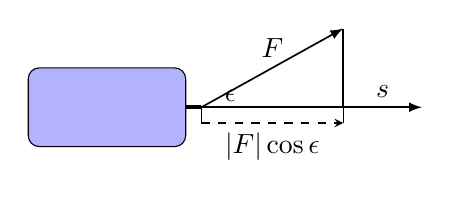
\begin{tikzpicture}
        \draw[fill=blue!30,rounded corners=4pt] (0,0.5) -- (-2,0.5) -- (-2,-0.5) -- (0,-0.5) --cycle;
        \draw[ultra thick] (0,0) -- (0.2,0);
        \draw[semithick] (0.2,0) -- (2,0);
        \draw[semithick, -latex] (2,0) -- node[above] {$\vv{s}$} (3,0);
        \draw[semithick, -latex] (0.2,0) -- node[above] {$\vv{F}$} (2,1);
        \draw[semithick] (2,0) -- (2,1);
        \node at (0.57,-0.05) [above] {$\epsilon$} ;
        \draw[] (0.2,0) -- (0.2,-0.2);
        \draw[] (2,0) -- (2,-0.2);
        \draw[dashed, stealth-,-stealth] (0.2,-0.2) --node[below] {$|\vv{F}| \cos{\epsilon}$} (2,-0.2);
    \end{tikzpicture}
    \caption{Ein Wagen auf einer Schiene wird durch eine seitwärts wirkende Kraft $\vv{F}$ nach rechts bewegt (Abbildung zum Beispiel \ref{example:arbeit})}
\end{marginfigure}
\begin{example}
Aus der Physik wissen wir, dass eine Kraft mechanische Arbeit verrichtet, wenn unter ihrer Wirkung ein Weg zurückgelegt wird. Wirkt beispielsweise auf einen Wagen, der sich auf einer Schiene befindet, seitwärts eine konstante Kraft $\vv{F}$, so gilt:
Die Arbeit $W$ ist das Produkt aus der längs der Schiene (Weg) wirkenden Komponente von $\vv{F}$ und dem zurückgelegten Weg $|\vv{s}|$, also:
\[ W = |\vv{F}||\vv{s}| \cos{\epsilon} \]
\label{example:arbeit}
\end{example}

\begin{definition}\index{Skalarprodukt}
Das \textit{Skalarprodukt} $\vv{a} \cdot \vv{b}$ zweier Vektoren $\vv{a}$ und $\vv{b}$ wird wie folgt festgelegt:
\[ \vv{a} \cdot \vv{b} = |\vv{a}| |\vv{b}| \cos{\epsilon} \]
wobei $\epsilon$ der Zwischenwinkel der beiden Vektoren ist.
\end{definition}
Als \textit{Zwischenwinkel} $\epsilon$ bezeichnet man den kleineren der beiden Winkel, die von Repräsentanten mit einem gemeinsamen Anfangspunkt eingeschlossen werden, d.h. $\SI{0}{\degree} \leq \epsilon \leq \SI{180}{\degree}$. Für zwei kollineare Vektoren ist der Zwischenwinkel \SI{0}{\degree} bei gleichem und \SI{180}{\degree} bei entgegengesetztem Richtungssinn.

\begin{margintable}[2.5cm]
    %\renewcommand{\arraystretch}{1.3}
    \centering
        \begin{tabular}{c|ccccccc}
        \toprule
            $\epsilon$   & \SI{0}{\degree} & \SI{30}{\degree} & \SI{60}{\degree} & \SI{90}{\degree} & \SI{120}{\degree} & \SI{150}{\degree} & \SI{180}{\degree} \\
            \midrule
            $\vv{a} \cdot \vv{b}$  & 12 & 10.4 & 6 & 0 & -6 & -10.4 & -12  \\
            \bottomrule
        \end{tabular}
        %\caption{Wahrscheinlichkeiten für die mit dem unfairen Würfel gewürfelten Augenzahlen (normiert auf 1)}
\end{margintable}

\begin{example}
Es seien $\vv{a}$ und $\vv{b}$ zwei Vektoren mit festen Beträgen $|\vv{a}| = 4$ und $|\vv{b}| = 3$. Wie verändert sich das Skalarprodukt $\vv{a} \cdot \vv{b}$, wenn der Zwischenwinkel $\epsilon$ variiert?
\end{example}

\begin{Vorzeichendsp}
Wir unterscheiden zwei Fälle:\newline
\begin{align*}
\text{Fall 1:} & &  \vv{a} = \vv{0} & \quad \text{ oder} & \vv{b} = \vv{0} & \quad \Rightarrow & \vv{a} \cdot \vv{b} = 0  & & \\
\text{Fall 2:} & &  \vv{a} \neq \vv{0} & \quad \text{ und} & \vv{b} \neq \vv{0} & \quad \Rightarrow & \vv{a} \cdot \vv{b} > 0 & \quad \Leftrightarrow & \SI{0}{\degree} \leq \epsilon < \SI{90}{\degree} \\
 & &  & &  &  & \vv{a} \cdot \vv{b} < 0 & \quad \Leftrightarrow & \SI{90}{\degree} < \epsilon \leq \SI{180}{\degree} 
\end{align*}
Also:
\[ \vv{a} \cdot \vv{b} = 0 \Leftrightarrow \vv{a} \text{ senkrecht} \vv{b} \]
\end{Vorzeichendsp}
Anders als beim Produkt von Zahlen, kann das Skalarprodukt $0$ sein, auch wenn keiner der beiden Faktoren ``null'' (d.h. Nullvektor) ist. Zwar sind, wie wir gleich sehen werden, durchaus Gemeinsamkeiten zwischen dem Zahlenprodukt und dem Skalarprodukt vorhanden. Dennoch bestehen auch wesentliche Unterschiede, allein schon deshalb, weil beim Zahlenprodukt sowohl die Operanden als auch die Resultate aus der gleichen ``Objektmenge'' stammen (es sind alles Zahlen), während beim Skalarprodukt die Operanden Vektoren und die Resultate Zahlen sind.

\section{Rechengesetze des Skalarprodukts}
\begin{theorem}[Kommutativgesetz]
Für zwei Vektoren $\vv{a}$ und $\vv{b}$ gilt:
\[ \vv{a} \cdot \vv{b} = x( \vv{a} \cdot \vv{b}) \]
Dies folgt unmittelbar aus der Definition
\end{theorem}

\begin{theorem}[Assoziativgesetz]
Für zwei Vektoren $\vv{a}$ und $\vv{b}$ gilt:
\[ (x \vv{a}) \cdot \vv{b} = \vv{b} \cdot \vv{a} \]
\end{theorem}
\begin{proof}
Sei $\epsilon$ der Zwischenwinkel von $\vv{a}$ und $\vv{b}$. Wir unterscheiden drei Fälle:
\begin{align*}
x=0: \quad & \text{Beide Seiten sind } 0 \\
x>0: \quad & (x\vv{a}) \cdot \vv{b} = |x \vv{a}| |\vv{b}| \cos{\epsilon} = |x| |\vv{a}| |\vv{b}| \cos{\epsilon}\\
           & = x ( |\vv{a}| |\vv{b}| \cos{\epsilon} ) = x (\vv{a} \cdot \vv{b} )\\
x<0: \quad & (x\vv{a}) \cdot \vv{b} = |x \vv{a}| |\vv{b}| \cos{(\SI{180}{\degree} - \epsilon)} = |x| |\vv{a}| |\vv{b}| -\cos{\epsilon}\\
           & = (-x) ( |\vv{a}| |\vv{b}| -\cos{\epsilon} ) = x (\vv{a} \cdot \vv{b} )
\end{align*}
\end{proof}

\begin{theorem}[Distributivgesetz]
Für drei Vektoren $\vv{a}$, $\vv{b}$ und $\vv{c}$ gilt:
\[ \vv{a} \cdot (\vv{b} + \vv{c}) = \vv{a} \cdot \vv{b} + \vv{a} \cdot \vv{c} \]
\end{theorem}
\begin{proof}
Wir betrachten die Ebenen $E_{1}$ und $E_{2}$, die auf dem Repräsentaten des Vektors $\vv{a}$ (mit Anfangspunkt $X$) senkrecht stehen und durch die Spitzen der Pfeile gehen, welche die Vektoren $\vv{b}$ bzw. $\vv{c}$ repräsentieren. Die Punkte $Y$  und $Z$ seien die Schnittpunkte von $\vv{a}$ mit $E_{1}$ respektive $E_{2}$. $\alpha$ sei der Winkel zwischen $\vv{a}$ und $\vv{b} + \vv{c}$, $\beta$ derjenige zwischen $\vv{a}$ und $\vv{b}$ und $\gamma$ derjenige zwischen $\vv{a}$ und $\vv{c}$. Für die linke und rechte Seite der zu beweisenden Beziehung folgt nun:
\begin{align*}
\text{Linke Seite:}\\
\vv{a} \cdot (\vv{b} + \vv{c}) & =  |\vv{a}| |\vv{b} + \vv{c}| \cos{\alpha} = |\vv{a}| \overline{XZ}  \\
\text{Rechte Seite:}\\
\vv{a} \cdot \vv{b} + \vv{a} \cdot \vv{c} & = |\vv{a}| |\vv{b}| \cos{\beta} + |\vv{a}| |\vv{c}| \cos{\gamma} = |\vv{a}| \overline{XY} + |\vv{a}| \overline{YZ} = |\vv{a}| (\overline{XY} + \overline{YZ} ) = |\vv{a}| \overline{XZ}  
\end{align*}
Beide Seiten sind demnach gleich. Allerdings haben wir stillschweigend spitze Zwischenwinkel $\beta$ und  $\gamma$ und damit auch $\alpha$ angenommen. In jenen Fällen, wo mindestens einer der beiden Winkel $\beta$ oder $\gamma$ nicht spitz ist, geht die Beweisführung bis auf ein Vorzeichen gleich.
\end{proof}

\begin{warning}
Ein weiteres ``Assoziativgesetz'' gilt nicht!
\[ \underbrace{(\vv{a} \cdot \vv{b} ) \vv{c}}_{\text{Reelles Vielfaches von } \vv{c}} \neq \underbrace{\vv{a} (\vv{b} \cdot \vv{c} )}_{\text{Reelles Vielfaches von } \vv{a}} \]
Sind $\vv{c}$ und $\vv{a}$ nicht kollinear und ist keiner der beiden Klammernausdrücke 0, so sind auch die reellen Vielfachen nicht kollinear und demnach verschieden.
\end{warning}
Im Wesentlichen darf man also weiterhin rechnen wie mit Zahlen; Skalarprodukte benehmen sich nicht genau gleich wie Zahlenprodukte aber problematische Terme mit Skalarprodukten , die drei oder mehr Faktoren (Vektoren) aufweisen, kommen bei uns kaum vor. Abgesehen von solchen Termen kann man auf Grund der bewiesenen Rechengesetze weiterhin rechnen wie mit Zahlen.

\begin{marginfigure}[3.5cm]
    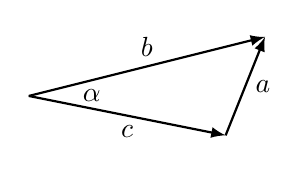
\begin{tikzpicture}
        \draw[-latex, thick] (0,0) --node[above] {$\vv{b}$} (3,0.75);
        \draw[-latex, thick] (0,0) --node[below] {$\vv{c}$} (2.5,-0.5);
        \draw[-latex, thick] (2.5,-0.5) --node[right] {$\vv{a}$} (3,0.75);
        \node at (0.8,0) {$\alpha$};
    \end{tikzpicture}
\end{marginfigure}
\begin{example}
Unter Verwendung eines Binoms ergibt sich:
\[ \vv{a}^{2} = (\vv{b}  \vv{c} )^{2} = \vv{b}^{2} - 2\vv{b} \cdot \vv{c} + \vv{c}^{2} \]
Aus der Gleichheit der links und rechts stehenden Terme und der Definition des Skalarproduktes folgt nun der Kosinussatz:
\[ |\vv{a}|^{2} = |\vv{b}|^{2} + |\vv{c}|^{2} - 2 |\vv{b}| |\vv{c}| \cos{\alpha} \]

\end{example}

\section{Das Skalarprodukt in der Komponentendarstellung}
\begin{theorem}\index{Skalarprodukt!Komponentendarstellung}
Für das Skalarprodukt zweier Vektoren $\vv{a}$ und $\vv{b}$ gilt in der Komponentendarstellung:
\[ \Vek{a_{1}}{a_{2}}{a_{3}} \cdot \Vek{b_{1}}{b_{2}}{b_{3}} = a_{1} b_{1} +  a_{2} b_{2} + a_{3} b_{3} \]
\end{theorem}

\begin{proof}
\begin{align*}
\skap{a}{b}  = & (a_{1} \vv{e_{1}} +a_{2} \vv{e_{2}} + a_{3} \vv{e_{3}}) \cdot (b_{1} \vv{e_{1}} +b_{2} \vv{e_{2}} + b_{3} \vv{e_{3}}) \\
  = &  a_{1} b_{1} \underbrace{\vv{e_{1}}^{2}}_{1} + a_{1} b_{2} \underbrace{\vv{e_{1}} \cdot \vv{e_{2}}}_{0} + a_{1} b_{3} \underbrace{\vv{e_{1}} \cdot \vv{e_{3}}}_{0} + \\
 & a_{2} b_{1} \underbrace{\vv{e_{2}} \cdot \vv{e_{1}}}_{0} + a_{2} b_{2} \underbrace{\vv{e_{2}}^{2}}_{1} + a_{2} b_{3} \underbrace{\vv{e_{2}} \cdot \vv{e_{3}}}_{0} + \\
 & a_{3} b_{1} \underbrace{\vv{e_{3}} \cdot \vv{e_{1}}}_{0} + a_{3} b_{2} \underbrace{\vv{e_{3}} \cdot \vv{e_{2}}}_{0} + a_{3} b_{3} \underbrace{\vv{e_{3}}^{2}}_{1} \\
 = & a_{1} b_{1} +  a_{2} b_{2} + a_{3} b_{3} 
\end{align*}
\end{proof}

\begin{example}
Die Betragsformel: \newline
Es gilt: $|\vv{a}| = \sqrt{\vv{a}^{2}} $. \newline
Ist nun $\vv{a} = \Vek{a_{1}}{a_{2}}{a_{3}}$, so folgt:
\[ |\vv{a}| = \sqrt{\Vek{a_{1}}{a_{2}}{a_{3}} \cdot \Vek{a_{1}}{a_{2}}{a_{3}}} = \sqrt{a_{1}^{2}+ a_{2}^{2} + a_{3}^{2}} \]
\end{example}

\section{Winkelformel}
Weil 
\[\skap{a}{b} = \left|\Vek{a_{1}}{a_{2}}{a_{3}} \right| \left|\Vek{b_{1}}{b_{2}}{b_{3}} \right| \cos{\epsilon}\]
ist, erhält man eine \textit{Winkelformel}:
\begin{theorem}\index{Zwischenwinkel zweier Vektoren}
Sei $\epsilon$ der Zwischenwinkel der beiden Vektoren $\vv{a}$ und $\vv{b}$, dann gilt für $\epsilon$:
\[ \epsilon = \arccos{\frac{\skap{a}{b}}{\left|\Vek{a_{1}}{a_{2}}{a_{3}} \right| \left|\Vek{b_{1}}{b_{2}}{b_{3}} \right|}} \]
\end{theorem}

%%%%%%%%%%%%%%%%%%%% Übungen %%%%%%%%%%%%%%%%%%%%%%%%%%


\begin{exercisesKapitel}
\begin{exercise}
$A=(2/1/0)$, $B=(3/-1/2)$, $C=(8/3/3)$  \newline Berechnen Sie den Winkel zwischen $\overline{AB}$ und $\overline{AC}$
\begin{answer}
\SI{67.6}{\degree}
\end{answer}
\end{exercise}

\begin{exercise}
$A=(1/1/1)$, $B=(3/3/2)$, $C=(4/1/4)$, $D=(2/-1/3)$  \newline Zeigen Sie, dass das Viereck $ABCD$ ein Quadrat ist.
\begin{answer}
Zu zeigen: $\vv{AB} = \vv{DC}$  und $|\vv{AB}| = |\vv{AD}|$ und $\vv{AB} \cdot \vv{AD} = 0$.
\end{answer}
\end{exercise}

\begin{exercise}
$A=(8/-2/-1)$, $B=(11/5/0)$, $C=(6/2/1)$ \newline
\begin{enumerate}
\item Zeigen Sie, dass das $ABC$ ein rechtwinkliges Dreieck ist.
\item Berechnen Sie den Winkel zwischen der Seite $a$ und der Seitenhalbierenden $s_{b}$.
\end{enumerate}
\begin{answer}
\begin{enumerate}
\item Zu zeigen: $\vv{CA} \cdot \vv{CB} = 0$ (der rechte Winkel ist also bei $C$).
\item \SI{22.5}{\degree}
\end{enumerate}
\end{answer}
\end{exercise}

\begin{exercise}
$A=(-1/0/2)$, $B=(-2/2/0)$, $C=(t/1+t/4-t)$ \newline
\begin{enumerate}
\item Berechnen Sie den Winkel zwischen den Vektoren $\vv{BA}$ und $\vv{BC}$ für $t=1$
\item Bestimmen Sie alle $t$ so, dass der Winkel zwischen den Vektoren $\vv{BA}$ und $\vv{BC}$ gleich \SI{45}{\degree} ist.
\end{enumerate}
\begin{answer}
\begin{enumerate}
\item \SI{45}{\degree}
\item $t=-11$ und $t=1$
\end{enumerate}
\end{answer}
\end{exercise}

\begin{exercise}
$\vv{a} = \Vek{x+1}{2-2x}{1}$, $\vv{b}=\Vek{x}{4}{2}$ \newline
Berechnen Sie $x$ so, dass $\vv{a}$ und $\vv{b}$ senkrecht aufeinander stehen.
\begin{answer}
$x_{1} = 2$, $x_{2} = 5$
\end{answer}
\end{exercise}

\begin{exercise}
Gegeben ist der Vektor $\vv{a} = \Vek{2}{-1}{-2}$ \newline
Berechnen Sie die Zwischenwinkel von $\vv{a}$ mit jedem der drei Basisvektoren.
\begin{answer}
Der Winkel zwischen $\vv{a}$ und $\vv{e_{1}} = \arccos{\frac{\vv{a}\cdot \vv{e_{1}}}{|\vv{a}| |\vv{e_{1}}|}} = \SI{48.2}{\degree}$ \newline
Der Winkel zwischen $\vv{a}$ und $\vv{e_{2}} = \arccos{\frac{\vv{a}\cdot \vv{e_{2}}}{|\vv{a}| |\vv{e_{2}}|}} = \SI{109.5}{\degree}$ \newline
Der Winkel zwischen $\vv{a}$ und $\vv{e_{3}} = \arccos{\frac{\vv{a}\cdot \vv{e_{3}}}{|\vv{a}| |\vv{e_{3}}|}} = \SI{131.8}{\degree}$
\end{answer}
\end{exercise}

%%%%%%%%%%%%%%%%%%%%%%%%%%%%%%%%%%%% https://www.sharelatex.com/project/54c7b9c3a50cfdaa3f0f6052


\begin{exercise}
$A=(1/1/1)$, $B=(7/4/3)$, $C=(-7/0/5)$ \newline
Wie gross sind die drei Winkel des Dreiecks $ABC$?
\begin{answer}
$\alpha=\SI{133.0}{\degree}$, $\beta=\SI{26.6}{\degree}$, $\gamma=\SI{20.4}{\degree}$
\end{answer}
\end{exercise}

\begin{exercise}
$A=(7/6/3)$, $B=(4/10/1)$, $C=(-2/6/2)$, $D=(1/2/4)$ \newline
Beweisen Sie, dass das Viereck $ABCD$ ein Rechteck ist.
\begin{answer}
Zu zeigen: $\vv{AB} = \vv{DC}$ (Parallelogramm), $\vv{AB} \cdot \vv{AD} = 0$ (Parallelogramm ist Rechteck)
\end{answer}
\end{exercise}

\begin{exercise}
$A=(2/3/-2)$, $B=(6/-1/1)$ \newline
Für welche Punkte $P$ der $x$-Achse ist der Winkel zwischen $\overline{PA}$ und $\overline{PB}$ gleich \SI{90}{\degree}?
\begin{answer}
$\vv{PA} \cdot \vv{PB} = 0$ mit $P=(x/0/0) \rightarrow P_{1} = (1/0/0)$, $P_{2}=(7/0/0)$
\end{answer}
\end{exercise}

\begin{exercise}
$A=(-2/1/4)$, $B=(1/-5/7)$, $C=(4/3/2)$, $D=(-1/5/11)$ \newline
\begin{enumerate}
\item Zeigen Sie, dass die von $A$ auslaufenden Kanten der Pyramide $ABCD$ paarweise senkrecht aufeinander stehen.
\item Berechnen Sie das Volumen $V$ der Pyramide.
\end{enumerate}
\begin{answer}
\begin{enumerate}
\item Zu zeigen: $\vv{AB} \cdot \vv{AC} = \vv{AB} \cdot \vv{AD} = \vv{Ac} \cdot \vv{AD} =0$
\item $V=\frac{1}{6} |\vv{AB}| |\vv{AC}| |\vv{AD}| = 66$
\end{enumerate}
\end{answer}
\end{exercise}

\begin{exercise}
Gegeben ist der Vektor $\vv{a} = \Vek{x}{8}{\sqrt{11}}$ \newline
Für welches $x$ schliessen die Vektoren $\vv{a}$ und $\vv{e_{1}}$ einen Winkel von \SI{60}{\degree} ein?
\begin{answer}
$x=5$
\end{answer}
\end{exercise}

\begin{exercise}
$A=(8/1/-1)$, $B=(2/4/-3)$ \newline
Im gleichschenkligen Dreieck $ABC$ mit Spitze $C$ liegt die Ecke $B$ auf der $y$-Achse. Bestimmen Sie $B$ und den Winkel $\alpha$.
\begin{answer}
$|\vv{CA}| = |\vv{CB}|$ mit $B=(0/y/0) \rightarrow B_{1} = (0/10/0)$, $B_{2} = (0/-2/0) \rightarrow \alpha_{1} = \SI{30.3}{\degree}$, $\alpha_{2} = \SI{52.1}{\degree}$
\end{answer}
\end{exercise}

\begin{exercise}
Ein Vektor schliess mit $\vv{e_{1}}$ einen Winkel von \SI{60}{\degree} und mit $\vv{e_{2}}$ einen Winkel von \SI{45}{\degree} ein. Welchen Winkel schliesst er mit $\vv{e_{3}}$ ein?
\begin{answer}
\SI{60}{\degree} oder \SI{120}{\degree} (Für den gesuchten Vektor den Betrag 1 annehmen und zweimal die Winkelfunktion verwenden)
\end{answer}
\end{exercise}

\begin{exercise}
$A=(3/3/3)$, $B=(5/1/4)$, $C=(3/0/6)$, $D=(1/2/5)$, \newline $E=(4/5/5)$, $F=(6/3/6)$, $G=(4/2/8)$, $H=(2/4/7)$ \newline
Zeigen Sie, dass diese acht Punkte die Ecken eines Würfels bilden.
\begin{answer}
$\vv{AB}=\vv{DC} = \vv{EF} = \vv{HG}$, $\vv{AD} = \vv{EH}$ (spat), $\vv{AB} \cdot \vv{AD} = \vv{AB} \cdot \vv{AE} = \vv{AD} \cdot \vv{AE} = 0$ (Spat ist Quader), $|\vv{AB}| = |\vv{AD}| = |\vv{AE}|$ (Quader ist Würfel)
\end{answer}
\end{exercise}

\begin{exercise}
Es sei $\vv{a} + \vv{b} - \vv{c} = \vv{0}$ und $|\vv{c}|=5$. Wie viel ist dann $\vv{a} \cdot \vv{c} + \vv{b} \cdot \vv{c}$?
\begin{answer}
$\vv{a} \cdot \vv{c} + \vv{b} \cdot \vv{c} = \vv{c} \cdot (\vv{a} + \vv{b} ) = \vv{c}^{2} = |\vv{c}|^{2} = 25$
\end{answer}
\end{exercise}

%%%%%%%%% ab Aufgabe 45 S.31 weiterfahren
\begin{exercise}
Für welche Vektoren gilt
\begin{enumerate}
\item $\vv{a} \cdot \vv{b} = |\vv{a}| |\vv{b}|$?
\item $|\vv{a} \cdot \vv{b}| = |\vv{a}| |\vv{b}|$?
\end{enumerate}
\begin{answer}
\begin{enumerate}
\item Kollineare Vektoren die gleich gerichtet sind
\item Kollineare Vektoren, die gleich oder entgegengesetzt gerichtet sind
\end{enumerate}
\end{answer}
\end{exercise}

\begin{marginfigure}[3cm]
    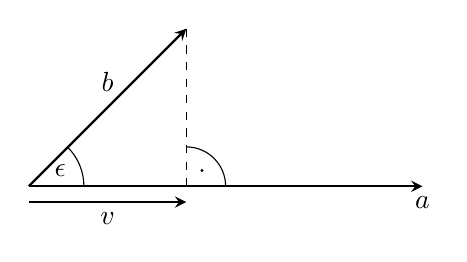
\begin{tikzpicture}
        \coordinate (O) at (0,0);
        \coordinate (A) at (2,2);
        \coordinate (B) at (5,0);
        \coordinate (C) at (2,0);
        \draw[-stealth,thick] (O) -- (B) node[below] {$\vv{a}$};
        \draw[-stealth,thick] (O) --node[above=2] {$\vv{b}$} (A);
        \draw[dashed] (A) -- (C);
        \draw (2.5,0) arc (0:90:0.5);
        \draw[fill=black] (2.2,0.2) circle (0.01);
        \draw[-stealth,thick] (0,-0.2) --node[below] {$\vv{v}$} (2,-0.2);
        \draw (0.7,0) arc (0:45:0.7);
        \node at (0.4,0.2) {$\epsilon$};
    \end{tikzpicture}
    \caption{Skizze zu Aufgabe (17)}
\end{marginfigure}

\begin{exercise}
Zeigen Sie für $\vv{v}$ gemäss Skizze:
\[ \vv{v} = \frac{\vv{a} \cdot \vv{b}}{|\vv{a}|^{2}} \vv{a} \]
Gilt diese Formel auch wenn $\epsilon$ stumpf ist?
\begin{answer}
\[ \vv{v} = |\vv{b}| \cos{\epsilon} \frac{1}{|\vv{a}|} \vv{a} = \frac{|\vv{a}| |\vv{b}|} \cos{\epsilon}{|\vv{a}|^{2}} \vv{a} =\frac{\vv{a} \cdot \vv{b}}{|\vv{a}|^{2}} \vv{a}\]
Die Formel ist auch für stumpfe Winkel $\epsilon$ gültig.
\end{answer}
\end{exercise}



\end{exercisesKapitel}